\section{Identification of the electrical energy}\label{sec:conductivity}

We now identify the energy seen by functions that vary on a fixed spatial
scale.  This will determine the Green kernel in the next section.  The
argument uses the cutoffs and circuit flows of
Theorem~\ref{thm:network-bounds}; its conclusion concerns locally uniform
convergence of functions and does not yet assert convergence of closed forms
on \(L^2\).

We work on a joint representation extraction as in
Proposition~\ref{prop:geometry}, enlarged by the numerical observations of
Proposition~\ref{prop:readout-extension}.  Write \(m\) for the extracted
time units; on a duration-one finite sphere \(m=2n\).  Fix an ordinary plane
chart \(D\) with an open buffer.  The same notation will be used for the
primal network and for the unit-conductance dual network.  A protected finite
graph containing every star needed in \(D\) represents the network there.
The conclusions are unchanged if this graph is enlarged, because every
smaller fixed test eventually has all of its incidences in the protection.

Let \(z_m(v)\) be the position of a network vertex in this chart.  Choose a
point \(z_m(e)\) on each embedded edge.  The maximum diameter of the stars
meeting a compact subset of \(D\) tends to zero.  In particular, moving
\(z_m(e)\) to either endpoint changes its position by a quantity tending
uniformly to zero.  For an open \(U\subset D\), put
\begin{equation}\label{eq:local-network-energy}
 \mathcal E_m(w;U)
   =\sum_{e:\,z_m(e)\in U}(d_e w)^2,
 \qquad d_e w=w(e^+)-w(e^-).
\end{equation}
Each unoriented edge is counted once, with multiplicity; loop terms vanish.
We write \(\mathcal E_m(w)\) for the energy on the whole retained graph.
In the primal sphere this is the restriction of \(\mathcal E_n^0\) from
Section~\ref{sec:model}.  All choices of edge locations give the same
interior limits below.

We shall repeatedly use the following precise consequence of
Theorem~\ref{thm:network-bounds}.  In every fixed circular collar with
prescribed relative widths and room in \(D\), there is a cutoff taking the
values \(1\) and \(0\) on the two prescribed sides, with energy bounded by a
constant depending only on those relative widths.  There is also a
probability law of simple surrounding circuits whose expected edge-count
traffic \(\tau\) satisfies \(\sum_e\tau(e)^2\le B\), with the same type of
bound.  The constants do not depend on the absolute radius.  The index
after which a bound holds may depend on the fixed collar and on the sample.
Every use below fixes finitely many collars before letting \(m\) tend to
infinity.

\subsection{A relaxation for locally uniform convergence}

For \(f\in C(U)\), an open \(V\Subset U\), and \(\varepsilon>0\), define
\begin{equation}\label{eq:constrained-energy}
 q_m(f,V,\varepsilon)
  =\inf\left\{\mathcal E_m(w;V):
       \abs{w(v)-f(z_m(v))}\le\varepsilon
       \text{ for every }v\text{ with }z_m(v)\in V\right\}.
\end{equation}
Here \(w\) is a real function on the protected graph.  Values at all other
vertices are free.  For sufficiently large \(m\), the buffer contains
every endpoint and incidence needed by the energy in \(V\).  The empty
vertex constraint is vacuous, and an infeasible finite constraint system
has infimum \(+\infty\).  Define two open-set functionals by
\begin{equation}\label{eq:uniform-relaxations}
 \begin{split}
 \mathcal R^-(f,U)
   &=\sup_{V\Subset U}\ \lim_{\varepsilon\downarrow0}
                     \liminf_{m\to\infty}q_m(f,V,\varepsilon),\\
 \mathcal R^+(f,U)
   &=\sup_{V\Subset U}\ \lim_{\varepsilon\downarrow0}
                     \limsup_{m\to\infty}q_m(f,V,\varepsilon).
 \end{split}
\end{equation}
The suprema are over open \(V\) with compact closure.  The tolerance limits
exist by monotonicity.  Taking inner domains is necessary because the
membership of an edge near a specified boundary can change when its
representative location is changed.

\begin{lemma}[Cell sandwich and recovery]\label{lem:uniform-relaxation}
After a further joint extraction of countably many cell-constrained
infima, \(\mathcal R^-=\mathcal R^+\) for every continuous \(f\) and every
relatively compact open \(U\subset D\), simultaneously.  Write
\(\mathcal R(f,U)\) for the common value.  It has the following properties.
\begin{enumerate}[label=\textup{(\roman*)}]
\item If \(w_m\) converges locally uniformly to \(f\) on \(U\), in the
vertex positions \(z_m\), then
\[
 \mathcal R(f,U)\le\liminf_m\mathcal E_m(w_m;U).
\]
\item If \(V\Subset W\Subset U\) and \(\mathcal R(f,U)<\infty\), there
are \(w_m\) converging uniformly to \(f\) on a neighborhood of
\(\overline W\) such that
\[
 \limsup_m\mathcal E_m(w_m;W)\le\mathcal R(f,U).
\]
\item If \(f_j\in C(U)\) and \(f_j\to f\) uniformly on \(W\), where
\(V\Subset W\Subset U\),
then
\[
 \mathcal R(f,V)\le\liminf_j\mathcal R(f_j,W).
\]
\end{enumerate}
The functional is determined by the retained local numerical outputs on
arbitrarily slightly larger domains.  Two protected descriptions give the
same functional on their common interior.
\end{lemma}

\begin{proof}
We first describe the numerical outputs.  A fixed intrinsic cell instruction
selects a finite set of counted edges from the exact incidence record.  It
also attaches a rational closed interval to each of finitely many cell
labels.  A vertex carrying several labels must satisfy all their intervals.
Take the infimum of the sum of squared differences on the selected edges
over all such vertex functions, and compactify its value by
\(s\mapsto s/(1+s)\), with \(+\infty\mapsto1\).  This is a measurable
function of a finite incidence record: the objective is a finite quadratic
polynomial and the constraints are finitely many closed intervals.  The
list of intrinsic cell instructions and rational intervals is countable.
Proposition~\ref{prop:readout-extension} therefore retains their joint
limits, including equality through a common union record on overlaps.

Fix \(V_0\Subset V_1\Subset U\) and
\(\varepsilon_0>\varepsilon_1>0\).  On the continuum activation event,
cover the full preimage of \(\overline V_0\) by finitely many used cells
whose closures lie over \(V_1\); include the complete stars of their
vertices and edges.  Subdivide the cells so that the oscillation of \(f\)
on each image is smaller than a fixed fraction of
\(\varepsilon_0-\varepsilon_1\).  Rational intervals can then be chosen
so that, for every represented vertex of that cell and all large \(m\),
\begin{equation}\label{eq:value-interval-sandwich}
 [f(z_m(v))-\varepsilon_1,f(z_m(v))+\varepsilon_1]
 \ \subset\ J_{\rm cell}\
 \subset\
 [f(z_m(v))-\varepsilon_0,f(z_m(v))+\varepsilon_0].
\end{equation}
The first inclusion holds for every label at a multiply labelled vertex,
so these simultaneous demands are compatible.  Full preimages, star mesh,
and the strict margins ensure that the selected edge set contains every
edge located in \(V_0\) and contains only edges located in \(V_1\).
The constrained vertex set contains every vertex located in \(V_0\) and
contains only vertices located in \(V_1\).

Let \(s_m\) be the resulting infimum.  The eventual exact-incidence and
activation conclusions of Proposition~\ref{prop:readout-extension}, followed
by \eqref{eq:value-interval-sandwich}, give
\begin{equation}\label{eq:infimum-sandwich}
 q_m(f,V_0,\varepsilon_0)\le s_m
       \le q_m(f,V_1,\varepsilon_1)
 \qquad\text{for all sufficiently large }m.
\end{equation}
The observation \(s_m\) was extracted before this activation was selected;
activation only supplies its interpretation in the spatial chart.  Its
limit exists in \([0,\infty]\).  Although \(f,V_0,V_1\) were arbitrary,
every instruction just used belongs to the one countable list.  Uniform
continuity of \(f\) on the relevant compact sets and the separated
tolerances are what allow that list to serve all continuous functions.
More precisely, each instruction's activation is defined from its local
continuum cells and margins alone; it does not use \(f\) or the value
intervals.  After \(f\) is given we choose a suitable entry among the
already activated countable entries.  This is a pathwise use of their
simultaneous conclusions, not a new conditioning event.

It follows from \eqref{eq:infimum-sandwich} that
\[
 \limsup_m q_m(f,V_0,\varepsilon_0)
 \le \liminf_m q_m(f,V_1,\varepsilon_1).
\]
For each inner \(V_0\) choose \(V_1\Subset U\), and choose
\(\varepsilon_1<\varepsilon_0\).  Taking the limits and suprema in
\eqref{eq:uniform-relaxations} gives
\(\mathcal R^+(f,U)\le\mathcal R^-(f,U)\).  The opposite inequality is
immediate.  The same sandwich shows that an alternative edge-location
convention or an overlapping protected record gives the same result.

For (i), on each fixed \(V\Subset U\) and at each positive tolerance,
\(w_m\) is eventually admissible in \eqref{eq:constrained-energy}.
Its energy on \(V\) is at most its energy on \(U\).  Take the liminf,
then the tolerance limit and the inner-domain supremum.

For (ii), choose \(W'\) with \(W\Subset W'\Subset U\).  For each fixed
\(\varepsilon>0\), the limsup of \(q_m(f,W',\varepsilon)\) is at most
\(\mathcal R(f,U)\).  Choose approximate minimizers and decrease
\(\varepsilon\) to zero sufficiently slowly with \(m\).  They converge
uniformly on \(W'\), and their energies on \(W'\), hence on \(W\), have the
asserted limsup.  This diagonal choice is made after the extracted sample
has been fixed; no new conditional law is asserted.

Finally, for fixed \(\varepsilon>0\) and all sufficiently large \(j\),
\[
 q_m(f,V',\varepsilon)
 \le q_m(f_j,V',\varepsilon/2)
 \quad\text{whenever }V'\Subset V,
\]
because \(f_j\to f\) uniformly on \(W\).  Taking the limsup in \(m\)
bounds the right side by \(\mathcal R(f_j,W)\).  Take the liminf in \(j\),
then the tolerance limit and the supremum over \(V'\Subset V\).  This is
(iii).
\end{proof}

We will prove the following identification.  The recovery assertion is
stated with room in the domain because that is the form used when replacing
harmonic voltages.

\begin{theorem}[Unit conductivity]\label{thm:conductivity}
From every joint geometric extraction one can further extract the local
numerical outputs so that the following holds almost surely.  For the
primal and the unit dual network, for every open \(U\) compactly contained
in an ordinary conformal chart, and every \(f\in C(U)\),
\begin{equation}\label{eq:unit-conductivity}
 \mathcal R(f,U)=\int_U\abs{\nabla f}^2\dd x.
\end{equation}
The right side is \(+\infty\) if \(f\notin H^1_{\rm loc}(U)\), and is
allowed to be infinite otherwise.  For relaxations obtained along extractions
of finite spherical maps, the same identity holds in the common canonical
coordinate on every coordinate domain; the integral is the unhalved conformal
Dirichlet integral.

In particular, every sequence converging locally uniformly to \(f\) has
the lower energy bound of Lemma~\ref{lem:uniform-relaxation}(i).  For
\(V\Subset W\Subset U\) with finite right side in
\eqref{eq:unit-conductivity}, there is a sequence of vertex functions
\(w_m\) converging uniformly to \(f\) on a neighborhood of
\(\overline W\), with limsup energy on \(W\) at most that right side.
The coefficient in
\eqref{eq:unit-conductivity} is the same for all extractions.
\end{theorem}

\subsection{The local quadratic energy}

We first establish the deterministic structure of \(\mathcal R\).  The
cutoffs in Theorem~\ref{thm:network-bounds} make it possible to combine
two uniform recoveries without a fixed loss in their energy.

\begin{lemma}[Gluing and energy measures]\label{lem:energy-measures}
Suppose \(f\in C(U)\) and \(\mathcal R(f,V)<\infty\) for every
\(V\Subset U\).  The values \(V\mapsto\mathcal R(f,V)\) are the open-set
values of a Radon measure \(\Gamma_f\) on \(U\).  These measures are local:
if \(f=g\) on an open set, their restrictions there agree.  They are
invariant under addition of constants.  For locally finite values they
satisfy
\begin{equation}\label{eq:measure-parallelogram}
 \Gamma_{f+g}+\Gamma_{f-g}=2\Gamma_f+2\Gamma_g,
 \qquad \Gamma_{af}=a^2\Gamma_f\quad(a\in\R).
\end{equation}
Consequently
\[
 \Gamma(f,g)=\tfrac14(\Gamma_{f+g}-\Gamma_{f-g})
\]
is a symmetric bilinear signed Radon measure.  For every relatively compact
Borel set \(E\),
\begin{equation}\label{eq:measure-cauchy-schwarz}
 \abs{\Gamma(f,g)(E)}^2\le\Gamma_f(E)\Gamma_g(E).
\end{equation}
\end{lemma}

\begin{proof}
Here is the gluing estimate, including the localization it needs.  Let a
compact set be covered by finitely many open recovery regions
\(U_1,\ldots,U_h\), with all closures and supports kept inside a larger
protected chart.  Choose finitely many smaller disks covering the compact
set, each with a fixed enlargement in one \(U_i\).  The disk cutoffs from
Theorem~\ref{thm:network-bounds}, followed by finite maxima, give functions
\(\eta_i\in[0,1]\) supported with room in \(U_i\), with
\(\sum_i\eta_i\ge1\) on a neighborhood of the compact set and with
bounded energies.  Dividing by their sum there gives weights
\(\theta_i\ge0\) with \(\sum_i\theta_i=1\).  Outside that neighborhood
one can divide by \(\max\{\sum_i\eta_i,1/2\}\).  On the bounded range of
these functions this operation is Lipschitz, so the energies of the
\(\theta_i\) are bounded by a fixed multiple of
\(\sum_i\mathcal E_m(\eta_i)\).

Let \(w_{i,m}\) approach \(f\) uniformly in the regions where \(\theta_i\)
is used, with common error \(\delta_m\to0\), and set
\(w_m=\sum_i\theta_i w_{i,m}\) near the compact set.  For a counted edge
\(e=(x,y)\) there, its endpoints lie in this neighborhood for large \(m\).
Using \(\sum_i d_e\theta_i=0\), we have
\begin{equation}\label{eq:edge-gluing}
 d_e w_m
 =\sum_i\theta_i(y)d_e w_{i,m}
   +\sum_i\bigl(w_{i,m}(x)-f(z_m(x))\bigr)d_e\theta_i.
\end{equation}
Jensen's inequality bounds the squared first term by
\(\sum_i\theta_i(y)(d_e w_{i,m})^2\).  The sum over edges of the square
of the second term is at most
\[
 h\delta_m^2\sum_i\mathcal E_m(\theta_i)=o(1).
\]
The cross term tends to zero by Cauchy--Schwarz whenever the energies of the
recoveries are bounded.  The support room and vanishing star mesh ensure
that every edge with a nonzero \(i\)-term belongs to the region where the
\(i\)-th recovery was estimated.  Thus gluing costs at most the sum of the
recovery energies plus \(o(1)\).

Monotonicity of \(\mathcal R(f,\cdot)\) is immediate, and its definition
gives inner regularity:
\[
 \mathcal R(f,O)=\sup_{V\Subset O}\mathcal R(f,V).
\]
For disjoint opens \(O_1,O_2\), use compactly contained test domains in
each.  The counted edge sets are disjoint, and the infimum with all the
constraints is at least the sum of the separate infima.  The liminf and
inner-domain limits give
\(\mathcal R(f,O_1\cup O_2)\ge
  \mathcal R(f,O_1)+\mathcal R(f,O_2)\).

For subadditivity, fix a compactly contained test domain in
\(O_1\cup O_2\).  Cover its closure by inset regions of \(O_1,O_2\),
recover \(f\) there using Lemma~\ref{lem:uniform-relaxation}(ii), and
apply \eqref{eq:edge-gluing}.  The glued functions converge uniformly on
the test domain, so Lemma~\ref{lem:uniform-relaxation}(i) bounds its
relaxation by \(\mathcal R(f,O_1)+\mathcal R(f,O_2)\).
Taking the inner supremum proves subadditivity.  The construction with
finitely many weights proves the corresponding finite-cover statement.
A compact subset of a countable open union has a finite subcover, so
inner regularity then gives countable subadditivity.

For clarity, these open-set facts give the asserted measure as follows.
For \(A\subset U\), take the infimum of \(\mathcal R(f,O)\) over open
\(O\supset A\).  Countable subadditivity makes this an outer measure.
If two sets have positive distance, disjoint open neighborhoods and
open-set superadditivity give the reverse additive inequality.  It is
therefore a metric outer measure, whose Borel restriction is a measure.
Its values on opens are \(\mathcal R(f,O)\) by monotonicity, and inner
regularity and local finiteness make it Radon.  This is the usual
open-set measure construction.

The constraints in an inner domain depend only on \(f\) there; this proves
locality.  Adding a constant to all vertex values proves invariance under
constants.  Also
\[
 q_m(af,V,\varepsilon)=a^2q_m(f,V,\varepsilon/\abs a)
 \quad(a\ne0),
\]
which proves homogeneity after relaxation.

To prove the parallelogram identity, first recover \(f\) and \(g\) on a
common smaller domain.  Their sums and differences converge uniformly
to \(f+g\) and \(f-g\), and the exact edge identity gives
\[
 \mathcal E_m(w_m+\widetilde w_m;V)
 +\mathcal E_m(w_m-\widetilde w_m;V)
 =2\mathcal E_m(w_m;V)+2\mathcal E_m(\widetilde w_m;V).
\]
Apply the two lower bounds on \(V\), the recovery upper bounds on a
slightly larger domain, and then exhaust the original open set.  This
gives
\(\Gamma_{f+g}+\Gamma_{f-g}\le2\Gamma_f+2\Gamma_g\) on opens and
also proves local finiteness of the sums.  Recover \(f+g\) and \(f-g\)
instead, and take their half-sum and half-difference.  The same displayed
identity gives the reverse inequality.  Equality on opens is equality of
Radon measures.  Polarization and homogeneity now give real bilinearity.
Finally, positivity of
\(\Gamma_{f+t g}(E)=\Gamma_f(E)+2t\Gamma(f,g)(E)+t^2\Gamma_g(E)\)
for every real \(t\) gives \eqref{eq:measure-cauchy-schwarz}.
\end{proof}

We record one consequence of the proof.  If a recovery \(w_m\) approaches
a function equal to a constant \(c\) on an open set \(O\), and
\(K\Subset O\), it can be made exactly \(c\) near \(K\) at a cost \(o(1)\)
in energy.  Indeed, take a bounded-energy cutoff \(\theta_m\) equal to
one near \(K\) and zero outside \(O\), and replace \(w_m\) by
\((1-\theta_m)w_m+\theta_m c\).  The error term in
\eqref{eq:edge-gluing} is bounded by the uniform error on \(O\) times
the cutoff gradient.  This modification is unchanged outside \(O\).
We will use it on the constant side strips of a square.

\begin{lemma}[Local Sobolev comparison]\label{lem:energy-bounds}
For every \(D_0\Subset D\) there are deterministic constants
\(0<c_{D_0}\le C_{D_0}<\infty\) such that, for every open
\(U\Subset D_0\),
\begin{equation}\label{eq:energy-comparison}
 c_{D_0}\int_U\abs{\nabla f}^2\dd x
 \le \mathcal R(f,U)
 \le C_{D_0}\int_U\abs{\nabla f}^2\dd x.
\end{equation}
For a continuous \(f\) outside \(H^1_{\rm loc}(U)\), the lower integral
is interpreted as \(+\infty\).  The upper bound first holds for smooth
\(f\), and holds also for
\(f\in C(U)\cap H^1_{\rm loc}(U)\).  Local finiteness of
\(\mathcal R(f,\cdot)\) for a continuous \(f\) implies
\(f\in H^1_{\rm loc}(U)\).  The inequalities also hold as inequalities
of measures on every subopen of \(D_0\).
\end{lemma}

\begin{proof}
For the upper bound, fix \(V\Subset U\) and a square grid of small fixed
spacing \(r\).  Cover a neighborhood of \(\overline V\) by disks of radius
comparable to \(r\), centered at grid points, with fixed enlargements
contained in \(U\).  Construct a cutoff partition
\((\theta_{i,m})\) as in the proof of Lemma~\ref{lem:energy-measures},
and put
\[
 w_{m,r}(v)=\sum_i f(x_i)\theta_{i,m}(v),
\]
where \(x_i\) is the center of the \(i\)-th disk.  At a vertex in \(V\),
all contributing centers are at distance \(O(r)\), so \(w_{m,r}\)
differs from \(f\) by at most its modulus of continuity at \(O(r)\).

For an edge in this region, subtract from the coefficients \(f(x_i)\)
the value at one contributing center.  The sum of the differences of
the partition weights is zero.  At most a fixed number of weights
contribute, and each coefficient difference is at most
\(Cr\sup_{B_i'}\abs{\nabla f}\) on a fixed enlargement \(B_i'\).
The cutoff energies and their normalization are bounded independently
of \(r\).  Summing the squared edge differences gives
\begin{equation}\label{eq:partition-energy}
 \mathcal E_m(w_{m,r};V)
 \le C\sum_{i:\,B_i'\cap V\ne\varnothing}
             r^2\sup_{B_i'}\abs{\nabla f}^2
 \qquad\text{for all sufficiently large }m.
\end{equation}
The bounded overlap includes all endpoint margins.  For smooth \(f\),
first let \(m\) tend to infinity with \(r\) fixed.  Then let \(r\)
decrease to zero.  The right side is bounded by the corresponding
Riemann estimate on any fixed intermediate open set between \(V\) and
\(U\), and hence by \(C\int_U\abs{\nabla f}^2\).
The uniform errors tend to zero.  The definition of \(\mathcal R\)
and inner exhaustion prove the upper bound.

For the lower bound, let \(w_m\to f\) locally uniformly on \(U\), and
pass to a subsequence on which
\(\mathcal E_m(w_m;U)\) tends to its finite liminf \(L\).  At grid
spacing \(r\), use at each grid point \(x_i\) a circular collar
\[
       \alpha r<\abs{x-x_i}<\beta r,
       \qquad \tfrac12<\alpha<\beta<1,
\]
with fixed inner and outer margins; for example one can take
\(\alpha=0.7\) and \(\beta=0.8\).
Restrict to grid cells in an inner part of \(U\), so every buffered
collar lies in \(U\).  A surrounding circuit contains the inner disk
in its Jordan interior and has that interior inside the outer disk.
For neighboring grid points the inner disks overlap, while each center
is outside the other's outer disk.  Thus two such circuits must
intersect: otherwise their overlapping interiors would be nested,
contrary to the center exclusion.  Circuits in the same embedded
network intersect at a graph vertex.

Let \(E_{i,m}\) be the energy of \(w_m\) in the buffered \(i\)-th collar.
If \(\tau_i\) is the expected counting traffic of its circuit law, then
\[
 \EE\!\left[\sum_{e\in\gamma_i}\abs{d_e w_m}\right]
   =\sum_e\tau_i(e)\abs{d_e w_m}
   \le \sqrt{B E_{i,m}}.
\]
Choose one circuit satisfying this bound and assign any one of its
vertex values \(a_{i,m}\) to \(x_i\).  At a common vertex of two
neighboring circuits,
\[
 \abs{a_{i,m}-a_{j,m}}^2
       \le 2B(E_{i,m}+E_{j,m}).
\]
Every grid point has at most four neighbors.  The enlarged collars have
a fixed overlap multiplicity \(M\), including the edge-location margins
for all large \(m\) at this fixed \(r\).  Hence
\begin{equation}\label{eq:grid-energy-bound}
 \sum_{i\sim j}\abs{a_{i,m}-a_{j,m}}^2
 \le 8B\sum_i E_{i,m}
 \le 8BM\,\mathcal E_m(w_m;U).
\end{equation}
The piecewise affine interpolation on a triangulation of the grid has
Dirichlet integral bounded by a fixed multiple of the left side.
Moreover
\[
 \abs{a_{i,m}-f(x_i)}
 \le \omega_f(Cr)+o_m(1)
\]
on each fixed compact part of \(U\), where \(\omega_f\) is the local
modulus of continuity.  With \(r\) fixed, take a subsequence of the
finitely many grid values and let \(m\) tend to infinity in
\eqref{eq:grid-energy-bound}.  Then refine \(r\).  The interpolants
converge uniformly to \(f\) on inner compact sets and have bounded
Sobolev energy there.  Weak compactness in \(H^1\) and lower
semicontinuity yield the weak gradient of \(f\) and
\[
 \int_V\abs{\nabla f}^2\dd x\le C L
 \qquad(V\Subset U).
\]
One may use a finite union of inner grid regions at each stage, with
the same overlap bound.  Exhausting \(U\) gives the lower inequality
for a uniformly convergent sequence.

Apply that inequality to the recoveries in
Lemma~\ref{lem:uniform-relaxation}(ii), and exhaust their inner
domains.  It gives the lower bound in \eqref{eq:energy-comparison}
and the assertion that locally finite relaxed energy supplies a local
\(H^1\) gradient.

If \(f\in C(U)\cap H^1_{\rm loc}(U)\), mollification on a buffered
subdomain gives smooth \(f_j\) converging uniformly and in \(H^1\)
on any smaller fixed region.  After multiplication by a smooth cutoff
equal to one on that smaller region, extend \(f_j\) by zero to \(U\);
thus the inputs in the next step belong to \(C(U)\).  Use
Lemma~\ref{lem:uniform-relaxation}(iii) on \(V\Subset W\Subset U\)
and the smooth upper bound on \(W\).  It gives
\(\mathcal R(f,V)\le C\int_W\abs{\nabla f}^2\).
Choose such \(W\) inside \(U\) and exhaust \(U\) by \(V\).
This proves the upper bound for continuous \(H^1_{\rm loc}\)
functions.  All estimates used the same constants on every subopen of
the fixed ambient \(D_0\), so Radon regularity gives the corresponding
measure inequalities.
\end{proof}

The use of many grid scales in this proof is sequential: a grid and all
of its collars are fixed before the network limit, and only then is the
grid refined.  This is why the fixed-test electrical theorem suffices here.

\begin{lemma}[Tensor representation and scalar form]\label{lem:energy-tensor}
For each network, in each joint extraction there is a deterministic
constant \(k>0\), possibly depending on the extraction and on the choice
of primal or dual, such that in every ordinary chart
\begin{equation}\label{eq:scalar-relaxation}
 \mathcal R(f,U)=k\int_U\abs{\nabla f}^2\dd x
 \qquad(f\in C(U)\cap H^1_{\rm loc}(U)).
\end{equation}
The formula is understood with infinite values on an exhaustion.
The corresponding probability-one local assertion transfers to
strict-interior sphere charts with the same constant and the same raw
energy units.
\end{lemma}

\begin{proof}
Work first inside \(D_0\Subset D\).  Polarize the energy measures of
the coordinate functions \(x_1,x_2\), and define
\[
 A_{ij}(x)=\frac{\dd\Gamma(x_i,x_j)}{\dd x}(x).
\]
The densities exist because the upper bound of
Lemma~\ref{lem:energy-bounds} dominates the measures of
\(x_i+x_j\) and \(x_i-x_j\) by Lebesgue measure.  Bilinearity makes
\(A\) symmetric.  For each \(p\in\mathbb Q^2\),
\[
 \Gamma_{p\cdot x}=p^{\mathsf T}A p\,\dd x,\qquad
 c_{D_0}\abs p^2\le p^{\mathsf T}A(x)p
          \le C_{D_0}\abs p^2
 \quad\text{for almost every }x.
\]
Intersecting the exceptional sets for rational \(p\) and using continuity
in \(p\) gives \(c_{D_0}I\le A\le C_{D_0}I\) almost everywhere.

Let \(f\in C(U)\cap H^1_{\rm loc}(U)\) and write
\(\Gamma_f=e_f\,\dd x\), as permitted by the upper bound.  The
measure Cauchy--Schwarz inequality has the corresponding density
inequality; this follows by applying it on Borel sets and differentiating.
For every rational \(p\), outside a null set depending on \(f,p\),
\[
 \begin{split}
 \abs{e_f-p^{\mathsf T}A p}
 &=\left|\frac{\dd\Gamma(f-p\cdot x,f+p\cdot x)}{\dd x}\right|\\
 &\le \sqrt{e_{f-p\cdot x}\,e_{f+p\cdot x}}
 \le C_{D_0}\abs{\nabla f-p}\abs{\nabla f+p}.
 \end{split}
\]
Use one full-measure set for all rational \(p\), and let \(p\) approach
\(\nabla f(x)\).  We obtain
\begin{equation}\label{eq:tensor-relaxation}
 \mathcal R(f,U)=\int_U\nabla f^{\mathsf T}A\nabla f\dd x.
\end{equation}
The construction on smaller subdomains of this coordinate chart agrees
on overlaps by locality,
so these matrices form a measurable locally elliptic field.

We next identify its randomness and coordinate dependence.  At every
Lebesgue point,
\begin{equation}\label{eq:tensor-germ}
 A_{ij}(z)=\lim_{r\downarrow0}
   \frac{\Gamma(x_i,x_j)(B(z,r))}{\pi r^2},
\end{equation}
and it is enough to use a countable sequence of radii.  Each open energy
in the numerator is obtained from the cell infima in
Lemma~\ref{lem:uniform-relaxation}, on inner domains within that ball.
Balls with arbitrary centers can themselves be exhausted by a countable
base of rational open sets.  Thus the density is jointly measurable in
\(z\) and the retained arrays, and is readable from arbitrarily small
strict neighborhoods of \(z\).  No outside minimizer enters this reading:
only endpoints of counted edges are used, and their full stars lie in
the slightly larger protected neighborhood.  The affine functions and
their sums in \eqref{eq:tensor-germ} are among the continuous tests
handled by the one countable cell library.

We check the coordinate action required for this germ.  Transporting an
intrinsic cell instruction by a translation or a rotation only relabels
its spatial domains and the scalar value intervals in the same exact
finite incidence record.  The quadratic polynomial on its edges is
unchanged.  The inner-domain and tolerance sandwich therefore transports
the open energy measures.  A translation adds constants to the coordinate
functions, while a rotation \(x\mapsto Rx\) sends their gradient vectors
by \(R\); hence the density matrix is transported by
\(A\mapsto RAR^{\mathsf T}\).  On overlapping disks the union records
of Proposition~\ref{prop:readout-extension} give the common restriction
of these measures.  Thus the shrinking-ball reading has the translation
and rotation actions, with common restrictions, required by
Lemma~\ref{lem:deterministic-germs}.

Apply Lemma~\ref{lem:deterministic-germs} to bounded transforms of the
three entries of \(A\).  It makes \(A(z)\) deterministic for almost every
deterministic \(z\), and transports that value under the intrinsic affine
coordinate changes.  A translation changes each coordinate function by
a constant, which leaves its energy measure unchanged.  The deterministic
matrix is consequently translation invariant almost everywhere, hence
constant in the ordinary chart.  Equivalently, invariance under the
countable rational translations and mollification on smaller domains
gives the same conclusion.  A rotation conjugates this constant matrix
by the rotation matrix.  For a quarter-turn \(R\), invariance reads
\(A=RAR^{\mathsf T}\).  A real symmetric \(2\)-by-\(2\) matrix with this
property has equal diagonal entries and zero off-diagonal entries.
Thus \(A=kI\), with deterministic \(k>0\).

The preceding assertion is a probability-one statement about activated
local outputs and local continuum data.  Proposition~\ref{prop:sphere-support}
transfers its null failure event from the ordinary input and the extended
kernel to each strict-interior sphere patch at its actual field height,
without changing the raw energy units.  Its countable atlas and separate
auxiliary area-pair marginals remove the auxiliary chart marks.  This
proves \eqref{eq:scalar-relaxation} in the sphere reference charts with
the same deterministic constant.  The argument is applied separately to
the primal and dual outputs.  We denote the resulting constants by
\(k_{\rm p}\) and \(k_{\rm d}\).
\end{proof}

The last lemma determines the form of the energy.  It remains to determine
its coefficient.  We first put both networks in the same coordinate, then
use an exact finite planar identity.

\subsection{The common coordinate and planar duality}

For the full finite sphere graph, define \(q_m^{\rm can}\) and
\(\mathcal R_{\rm can}^{\pm}\) by
\eqref{eq:constrained-energy}--\eqref{eq:uniform-relaxations}, using the
canonical vertex and edge positions and using the full graph as the
protected graph.  Write \(\mathcal R_{\rm ref}\) for the relaxation in
a reference chart.

Let \(T_m=\phi_n\circ \Psi_n^{-1}\) be a comparison map from a reference
sphere to the canonical coordinate.  On the further extraction in
Proposition~\ref{prop:geometry}, \(T_m\to T\) uniformly, with \(T\)
conformal or anticonformal.  For fixed inner and outer domains,
uniform convergence gives the required inclusions of their images for
all large \(m\).  For a continuous \(f\), it also gives
\(f\circ T_m\to f\circ T\) uniformly on compact sets.  Applying the
domain and tolerance sandwich of Lemma~\ref{lem:uniform-relaxation}
in both directions therefore proves
\begin{equation}\label{eq:coordinate-relaxation}
 \mathcal R_{\rm can}(f,U)
   =\mathcal R_{\rm ref}(f\circ T,T^{-1}U).
\end{equation}
This argument uses only uniform convergence of \(T_m\); it does not require
convergence of their derivatives.  The two-dimensional scalar Dirichlet
integral is invariant under both conformal and anticonformal changes.
Thus the constants in Lemma~\ref{lem:energy-tensor} are unchanged in the
canonical coordinate.

We will also use the fixed cutoff and circuit tests in this coordinate.
On a sufficiently small compact neighborhood, the smooth map \(T\)
sends suitable reference collars inside and outside any fixed canonical
round collar, with all relative widths in a fixed bounded range.
Uniform convergence of \(T_m\) and the strict room between these collars
preserve their inclusions for all large \(m\).  The reference cutoffs
and circuits from Theorem~\ref{thm:network-bounds} therefore provide
canonical cutoffs and circuits with the same type of bounds, independent
of the absolute radius.  Each collar and its room are fixed before the
network limit; no simultaneous assertion at the mesh scale is used.

Use the dual rooted experiment of Lemma~\ref{lem:dual-geometry} in the
same joint extraction.  Its law, its number of edges, and its raw units
are those of the original rooted experiment.  Its primal scalar is
therefore \(k_{\rm p}\): both are deterministic marginal limits of the
same local output laws on this subsequence.  Its primal edges are the
original dual edges in the same physical flag surface, with the same
canonical marks.  After identifying the flag surfaces, we evaluate both
copies of this edge network through the original \(\phi_n\), using the
same physical edge representatives.  By three-point normalization, the
dual-rooted uniformization is either \(\phi_n\) or
\(\overline{\phi_n}\); in the latter case postcompose it with complex
conjugation to use the chosen coordinate.  Conjugation fixes
\(0,1,\infty\) and preserves the scalar Dirichlet integral.
On any common ordinary interior, the two canonical
relaxations of those edges are identical by their definition and
\eqref{eq:coordinate-relaxation}.  One reads \(k_{\rm d}\) in the first
experiment and \(k_{\rm p}\) in the second.  Consequently
\begin{equation}\label{eq:equal-dual-scalars}
                         k_{\rm p}=k_{\rm d}.
\end{equation}
Only the marginal probability-one conclusions are intersected here;
no independence between the two experiments is required.

The remaining scalar calculation is the planar self-duality fixed-point
method of Dykhne~\cite[Section~2]{Dykhne1971}.  The preceding work supplies
the existence, determinism, isotropy, and common-coordinate equality of
the two scalar limits needed here.  We now prove the complementary finite
identity and justify its passage to those limits.  For the finite
reciprocity statement compare Binder and Pechersky
\cite[Remark~2.11]{BinderPechersky2025}; the following proof includes the
contraction needed for our multigraph and boundary conventions.

\begin{lemma}[Complementary boundary conductances]\label{lem:mixed-duality}
Let \(G\) be a finite connected planar multigraph in a closed disk whose
boundary is a simple cycle.  Split that cycle into four nonempty edge paths
\(D_0,N_0,D_1,N_1\) in cyclic order, with four distinct joining vertices.
Give every edge a conductance \(c_e>0\).  Let
\[
 C_{\rm p}
 =\min\left\{\sum_{e\in E(G)}c_e(d_e u)^2:
             u=0\text{ on }D_0,\quad u=1\text{ on }D_1\right\}.
\]
The endpoints of each prescribed arc are included in its constraint.

Form a dual graph with one vertex for each interior face and two additional
vertices \(b_0,b_1\).  Each interior edge has its usual dual, with
conductance \(c_e^{-1}\).  A boundary edge on \(N_i\) has a dual edge
from its interior face to \(b_i\), with conductance \(c_e^{-1}\).
Discard duals of boundary edges on \(D_0,D_1\).  Let \(C_{\rm d}\) be
the minimum dual energy with values \(0,1\) at \(b_0,b_1\).  Then
\begin{equation}\label{eq:finite-duality}
                              C_{\rm p}C_{\rm d}=1.
\end{equation}
The statement permits loops, parallel edges, and repeated face incidences.
\end{lemma}

\begin{proof}
Contract each prescribed arc to a vertex, denoted \(t\) for value \(0\)
and \(s\) for value \(1\), and delete the contracted boundary edges.
The two remaining boundary paths run from \(s\) to \(t\).  Add one
\(s\)-to-\(t\) edge through the exterior, splitting the exterior into
two faces adjacent to \(N_0,N_1\).  This is a connected map on the sphere.

Let \(u\) minimize the primal unit-voltage energy and let \(I\) be its
total current out of \(s\).  It is harmonic at every free vertex.
Summation by parts gives
\[
 \sum_e c_e(d_eu)^2
   =\sum_v u(v)(Q_cu)(v)=I,
\]
so \(C_{\rm p}=I>0\).  Orient the original edges and put their signed
currents \(c_e\) times the corresponding voltage drops on them.  Put the
balancing current on the added exterior edge.  The resulting flow has
zero divergence at every vertex.

A divergence-free flow on a spherical planar map is the gradient of a
potential on its faces, with the dual orientation convention.  To see
this directly, integrate the flow across a dual path from a fixed face.
Two choices of dual path differ by cuts enclosing vertices; the integral
around each such cut is the sum of the divergences it encloses, hence
zero.  This defines a face potential \(\psi\), unique up to a constant.
Its potential drop between the two exterior faces has magnitude \(I\),
because their separating dual edge crosses the added edge.

On the dual of an original edge, multiplication of this face-potential
difference by \(c_e^{-1}\) gives the corresponding primal voltage
difference.  These dual currents have zero divergence at an interior face:
the primal voltage differences telescope around its boundary, including
repeated incidences.  At the two exterior faces their total currents have
magnitude \(1\), the voltage difference between \(s\) and \(t\) along
either boundary path.  Removing the dual of the added edge thus gives a
dual current of magnitude \(1\) at voltage drop \(I\).  Rescaling to
unit dual voltage gives \(C_{\rm d}=1/I\).

The contracted map has exactly the dual described in the statement.
An interior chord whose endpoints were contracted together is a loop and
has zero primal voltage drop; its dual carries zero current in this
construction.  A primal loop and a dual loop are handled by the same
incidence and telescoping identities.  Thus no simplicity beyond the
boundary cycle was used.
\end{proof}

\begin{figure}[t]
 \centering
 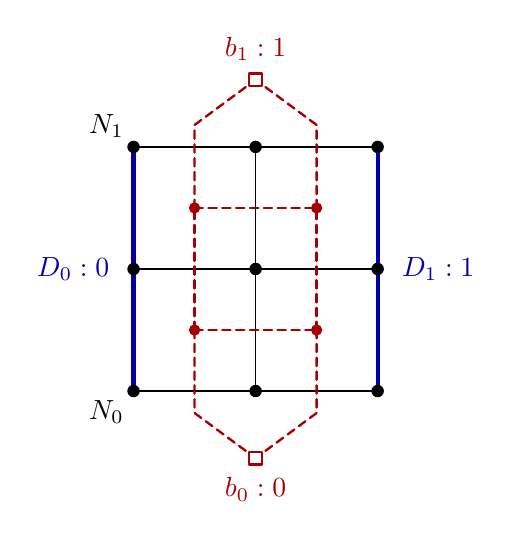
\begin{tikzpicture}[scale=1.55, line cap=round, line join=round,
    primal/.style={draw=black, line width=.65pt},
    prescribed/.style={draw=blue!65!black, line width=1.5pt},
    dual/.style={draw=red!65!black, densely dashed, line width=.85pt},
    face/.style={circle, fill=red!65!black, inner sep=1.45pt},
    wire/.style={rectangle, draw=red!65!black, fill=white,
                 line width=.9pt, inner sep=2.3pt}]
  \draw[primal] (0,0) grid (2,2);
  \draw[prescribed] (0,0)--(0,2);
  \draw[prescribed] (2,0)--(2,2);

  \draw[dual] (.5,.5)--(1.5,.5);
  \draw[dual] (.5,1.5)--(1.5,1.5);
  \draw[dual] (.5,.5)--(.5,1.5);
  \draw[dual] (1.5,.5)--(1.5,1.5);
  \draw[dual] (.5,.5)--(.5,-.18)--(1,-.55);
  \draw[dual] (1.5,.5)--(1.5,-.18)--(1,-.55);
  \draw[dual] (.5,1.5)--(.5,2.18)--(1,2.55);
  \draw[dual] (1.5,1.5)--(1.5,2.18)--(1,2.55);

  \foreach \x in {0,1,2}
    \foreach \y in {0,1,2}
      \fill[black] (\x,\y) circle (1.45pt);
  \foreach \x in {.5,1.5}
    \foreach \y in {.5,1.5}
      \node[face] at (\x,\y) {};
  \node[wire] at (1,-.55) {};
  \node[wire] at (1,2.55) {};

  \node[left, text=blue!65!black] at (-.12,1) {\(D_0:0\)};
  \node[right, text=blue!65!black] at (2.12,1) {\(D_1:1\)};
  \node[below left] at (0,0) {\(N_0\)};
  \node[above left] at (0,2) {\(N_1\)};
  \node[below, text=red!65!black] at (1,-.63) {\(b_0:0\)};
  \node[above, text=red!65!black] at (1,2.63) {\(b_1:1\)};
\end{tikzpicture}

 \caption{The complementary boundary problems in
 Lemma~\ref{lem:mixed-duality}, shown on a \(2\)-by-\(2\) grid.
 The solid primal graph has prescribed values on \(D_0,D_1\).
 Dashed dual edges crossing the other two boundary arcs end at the two
 separate wired vertices \(b_0,b_1\); duals of the prescribed boundary
 edges are omitted.  The wiring represents the two exterior faces after
 the added source-to-sink edge splits the exterior.}
 \label{fig:mixed-boundary-duality}
\end{figure}

The finite identity will be used on squares whose boundary is an actual
primal circuit.  We first give the compactness fact needed for the lower
conductance bound.

\begin{lemma}[Local harmonic compactness]\label{lem:harmonic-compactness}
Let \(O\) be an open coordinate region in the extracted networks.  Suppose
\(w_m\) is harmonic at every vertex with full star in \(O\), and for every
\(V\Subset O\),
\(\sup_m\mathcal E_m(w_m;V)<\infty\).
Then \(w_m\) is asymptotically equicontinuous on compact subsets of \(O\):
if \(z_m(v_m),z_m(v_m')\) lie in a fixed compact subset and their distance
tends to zero, then
\(\abs{w_m(v_m)-w_m(v_m')}\to0\).
If the values are also locally bounded, every subsequence has a further
subsequence converging locally uniformly in vertex tests to a continuous
function.
\end{lemma}

\begin{proof}
Suppose two close vertex sequences have a common limiting position \(z\).
Choose a closed disk about \(z\) inside \(O\) and let \(M\) bound the energy
in a slightly larger disk.  For an integer \(N\), place \(N\) disjoint
concentric collars of the same relative shape inside that larger disk.
Their radii decrease geometrically, and they are all fixed before taking
the network limit.  In collar \(i\), the circuit-traffic estimate selects
a surrounding circuit \(\gamma_i\) with total variation at most
\(\sqrt{B E_{i,m}}\), where \(E_{i,m}\) is the energy paid in that collar.
The collars, including their fixed small margins, can be disjoint, so
some \(i\) has \(E_{i,m}\le M/N\).

Every vertex in the disk inside that circuit has value between the minimum
and maximum on the circuit.  Indeed all its undetermined vertices are
harmonic, and every component inside reaches the circuit: an original
graph path from such a component to the rest of the connected map must
meet the separating circuit.  The finite maximum principle therefore
bounds the oscillation inside by \(\sqrt{BM/N}\).
For all sufficiently large \(m\), both close vertices lie inside the
smallest of the \(N\) collars.  Let \(m\) tend to infinity and then let
\(N\) increase.  This proves their difference tends to zero.  For a
random \(z\), the collars may be chosen from the countable library by
rational perturbations that keep a common inner disk and the disjoint
margins; their relative shapes remain in one fixed bounded range.

The sequential assertion gives equicontinuity on every compact by
contradiction and compactness of its position set.  The vertex positions
are dense in each compact region up to an error tending to zero, by the
flag mesh and the homeomorphisms.  Choose vertices approaching a countable
dense set, extract their bounded values diagonally, and use the
equicontinuity to extend the limits continuously and uniformly on finite
nets.  This gives the stated local uniform convergence.
\end{proof}

\begin{lemma}[Conductance of an approximating square]\label{lem:square-conductance}
Let \(Q=(0,1)^2\) have closure in an ordinary canonical chart.  There are
simple primal boundary circuits approaching \(\partial Q\), with four
ordered side arcs, for which the primal left-to-right and complementary
dual bottom-to-top conductances satisfy
\[
                C_m^{\rm p}\longrightarrow k_{\rm p},
 \qquad        C_m^{\rm d}\longrightarrow k_{\rm d}.
\]
The complementary dual uses exactly the wiring of
Lemma~\ref{lem:mixed-duality}.
\end{lemma}

\begin{proof}
Embed a cube graph in the canonical sphere with one facial cycle equal to
\(\partial Q\), and pull this embedding back to the reference sphere by
\(T^{-1}\).  The cubic skeleton lift
\cite[Lemma~4.7]{C} gives a subdivided primal cube whose graph
homeomorphism tracks the pulled-back embedding to any fixed accuracy; its facial
cycles and their order are preserved up to one reversal.
The reference homeomorphisms in Proposition~\ref{prop:geometry} have
vanishing projection error, and \(T_m\to T\) uniformly transfers that
tracking to the canonical sphere.  Apply the lift at successively smaller fixed
accuracies and choose their thresholds increasingly.  This gives a simple
primal cycle \(\gamma_m\) with an ordered parametrization approaching
\(\partial Q\) uniformly.  In particular, its inside contains every
compact subset of \(Q\) eventually and lies in every fixed enlargement
of \(\overline Q\).  Let \(G_m^Q\) be the submap consisting of this cycle
and everything inside it.  Its four arcs follow the four square sides
with error tending to zero.  Define \(C_m^{\rm p},C_m^{\rm d}\) as in
Lemma~\ref{lem:mixed-duality}, using unit conductances.

Write \(Q^\epsilon=\{x:\dist(x,\overline Q)<\epsilon\}\).  For an upper
bound, choose a smooth function \(f_\delta\) on a neighborhood
of \(\overline Q\), depending only on the horizontal coordinate, equal to
zero in a strip about the left side and one in a strip about the right
side.  It can be chosen with
\[
 \int_Q\abs{\nabla f_\delta}^2\dd x\longrightarrow1
 \quad\text{as }\delta\downarrow0.
\]
For example, flatten the linear function in strips of width \(\delta\),
use slope \(1/(1-2\delta)\) between them, and smooth the two bends in
smaller strips.  Extend it to a fixed small enlargement \(Q^\epsilon\).
For fixed \(\delta,\epsilon\), every edge of \(G_m^Q\) is eventually
located in \(Q^{\epsilon/2}\).  Apply the recovery clause of
Lemma~\ref{lem:uniform-relaxation} with
\(W=Q^{\epsilon/2}\Subset U=Q^\epsilon\), together with
\eqref{eq:scalar-relaxation}.  It recovers \(f_\delta\) uniformly on
a neighborhood of \(\overline{Q^{\epsilon/2}}\), with limsup energy
on \(Q^{\epsilon/2}\) at most
\(k_{\rm p}\int_{Q^\epsilon}\abs{\nabla f_\delta}^2\dd x\).
The constant-recovery modification after
Lemma~\ref{lem:energy-measures} makes it exactly zero and one on smaller
side strips, with additional energy \(o(1)\).  The boundary arcs lie
in these strips for all large \(m\).  Hence
\[
 \limsup_m C_m^{\rm p}
 \le k_{\rm p}\int_{Q^\epsilon}\abs{\nabla f_\delta}^2\dd x.
\]
Let \(\epsilon\downarrow0\), and then \(\delta\downarrow0\), to obtain
\(\limsup C_m^{\rm p}\le k_{\rm p}\).

For the dual upper bound use the corresponding function of the vertical
coordinate, with the same recovery domains
\(W=Q^{\epsilon/2}\Subset U=Q^\epsilon\).  Thus the full-dual recovery
converges uniformly on a neighborhood of
\(\overline{Q^{\epsilon/2}}\), and its limsup energy on \(Q^{\epsilon/2}\)
is bounded by \(k_{\rm d}\) times its Dirichlet integral over \(Q^\epsilon\).
Apply the constant-recovery modification after
Lemma~\ref{lem:energy-measures} to this full-dual recovery on smaller
bottom and top side strips whose closures lie in \(Q^{\epsilon/2}\)
and in the constant regions of the vertical profile.  It makes the
recovery exactly zero and one there, with additional energy \(o(1)\).
Give an interior face its modified full-dual value and
give each wired vertex its prescribed constant.  A dual edge crossing
one of the two relevant boundary arcs has its other endpoint at a
genuine exterior face of the full map.  The complete star of that face
has diameter tending to zero.  Thus this endpoint is in the smaller
constant side strip for all large \(m\), and the squared difference is
exactly the squared difference to the wired value.  The same face cannot
meet the two separated side strips.  For this fixed \(\epsilon\), all
interior dual edges and these boundary crossing edges eventually lie in
\(Q^{\epsilon/2}\), including their whole
endpoint stars.  Their energy is consequently bounded by the recovered
full-dual energy on \(Q^{\epsilon/2}\).  The identical sequence of fixed
limits, with vertical \(f_\delta\), gives
\(\limsup C_m^{\rm d}\le k_{\rm d}\).

For the lower bound take a subsequence attaining the liminf of either
conductance and its minimizing voltages, clipped to \([0,1]\).
The upper bound just proved gives bounded total energies.
The voltages are harmonic at every undetermined vertex in the submap.
On each compact subset of \(Q\), the boundary is absent for large \(m\),
and all original primal incidences, or all original dual incidences, are
present.  Lemma~\ref{lem:harmonic-compactness} therefore gives a locally
uniformly convergent further subsequence, with continuous limit \(f\).

We verify its prescribed boundary values away from the four corners.
Near the relative interior of a primal prescribed side, extend the
voltage to its fixed value on all exterior vertices.  Locally this
adds no energy: an edge leaving the submap passes through a prescribed
boundary vertex.  Near a prescribed side for the dual problem, extend
the voltage to the wired value on the actual exterior faces.  The
boundary crossing edges in this neighborhood are precisely the edges
to that wired vertex in the complementary problem.  Other exterior
edges have both endpoints at the same value.  Whole-face mesh and the
positive distance from the corners ensure that no other side enters
this neighborhood.  Thus the extended energies in a fixed neighborhood
are bounded by the already bounded submap energies.

Fix a point in the relative interior of such a side.  Use \(N\) disjoint
fixed circular collars centered there, as in
Lemma~\ref{lem:harmonic-compactness}, within the neighborhood just
described.  Every surrounding circuit visits the exterior side of the
approximating boundary.  Its Jordan interior contains an inner disk;
a ray from a point of that disk on the exterior side to the far exterior
must cross the circuit.  The crossing has a fixed positive distance
from the limiting side, so vanishing mesh supplies an exterior vertex
of the circuit.  That vertex has the prescribed value.  One of the
\(N\) circuits has variation at most \(\sqrt{BM/N}\).  The maximum
principle inside it applies to all undetermined vertices; the other
vertices there have the prescribed constant value.  It bounds their
difference from that constant by \(\sqrt{BM/N}\).  First take the network
limit and then increase \(N\).  This proves that \(f\) extends
continuously to the prescribed value on each relative side interior,
uniformly on its compact subsegments.

For \(V\Subset Q\), all edges located in \(V\) belong to the submap
eventually, for either network.  Extend the minimizing function arbitrarily
outside the submap; no edge in this inner test sees the extension.
The lower relaxation bound and \eqref{eq:scalar-relaxation} give
\[
 k_{\rm p}\int_V\abs{\nabla f}^2\dd x
       \le\liminf_m C_m^{\rm p}
\]
in the primal case, and the corresponding inequality with \(k_{\rm d}\)
in the dual case.  Exhausting \(Q\) puts \(f\) in \(H^1(Q)\) when the
liminf is finite.  In the primal case its boundary values are zero and
one on the relative interiors of the left and right sides.  The Sobolev
line property and Cauchy--Schwarz on horizontal slices give
\(\int_Q\abs{\nabla f}^2\ge1\).  More explicitly, on
\(y\in[\eta,1-\eta]\) the boundary convergence makes
\(f(a,y)\) uniformly close to zero and \(f(1-a,y)\) uniformly close
to one for small \(a>0\).  For almost every such \(y\),
\[
 \int_a^{1-a}\abs{\partial_x f(x,y)}^2\dd x
 \ge \frac{\abs{f(1-a,y)-f(a,y)}^2}{1-2a}.
\]
Integrate, let \(a\downarrow0\), and then \(\eta\downarrow0\).
The dual problem has the same calculation on vertical slices.
Consequently both liminfs are at least their stated scalars.  Together
with the upper bounds this proves the lemma.
\end{proof}

\begin{proof}[Proof of Theorem~\ref{thm:conductivity}]
Lemma~\ref{lem:energy-tensor} identifies the two reference relaxations
with the scalar integrals \(k_{\rm p}\) and \(k_{\rm d}\).
Equation~\eqref{eq:coordinate-relaxation} puts these integrals in the
same canonical coordinate, and \eqref{eq:equal-dual-scalars} equates
their positive constants.  Apply Lemma~\ref{lem:mixed-duality} to every
submap in Lemma~\ref{lem:square-conductance}.  Its exact identity and
the two limits give
\[
                  k_{\rm p}k_{\rm d}=1.
\]
Thus \(k_{\rm p}=k_{\rm d}=1\).

For a continuous function outside \(H^1_{\rm loc}\), local finiteness
is ruled out by Lemma~\ref{lem:energy-bounds}.  For a continuous
\(H^1_{\rm loc}\) function with infinite integral, inner exhaustion
and its lower bound give infinite relaxed energy.  This completes
\eqref{eq:unit-conductivity} for every continuous input.

Proposition~\ref{prop:geometry}(iv) supplies ordinary chart interiors
from two rerootings covering the canonical sphere.  Each carries the
formula just proved, by Proposition~\ref{prop:sphere-support} in its
own marked marginal and by \eqref{eq:coordinate-relaxation}.  On
overlaps these are restrictions of the same finite-network relaxation,
as in Lemma~\ref{lem:uniform-relaxation}.  The Radon measure property
therefore patches their common Dirichlet density across a finite
subcover of each compact test.  This proves the sphere statement,
including at points omitted by one of the rootings.  The lower and
recovery assertions are Lemma~\ref{lem:uniform-relaxation} with the
now identified value.  Since the finite product has fixed the value
to one on every further extraction, the coefficient is independent
of the extraction.
\end{proof}
